\section{lib/efreet\_\-icon.h File Reference}
\label{efreet__icon_8h}\index{lib/efreet\_\-icon.h@{lib/efreet\_\-icon.h}}


\subsection{Detailed Description}
Contains the structures and methods used to support the FDO icon theme specificiation. 





This graph shows which files directly or indirectly include this file:\nopagebreak
\begin{figure}[H]
\begin{center}
\leavevmode
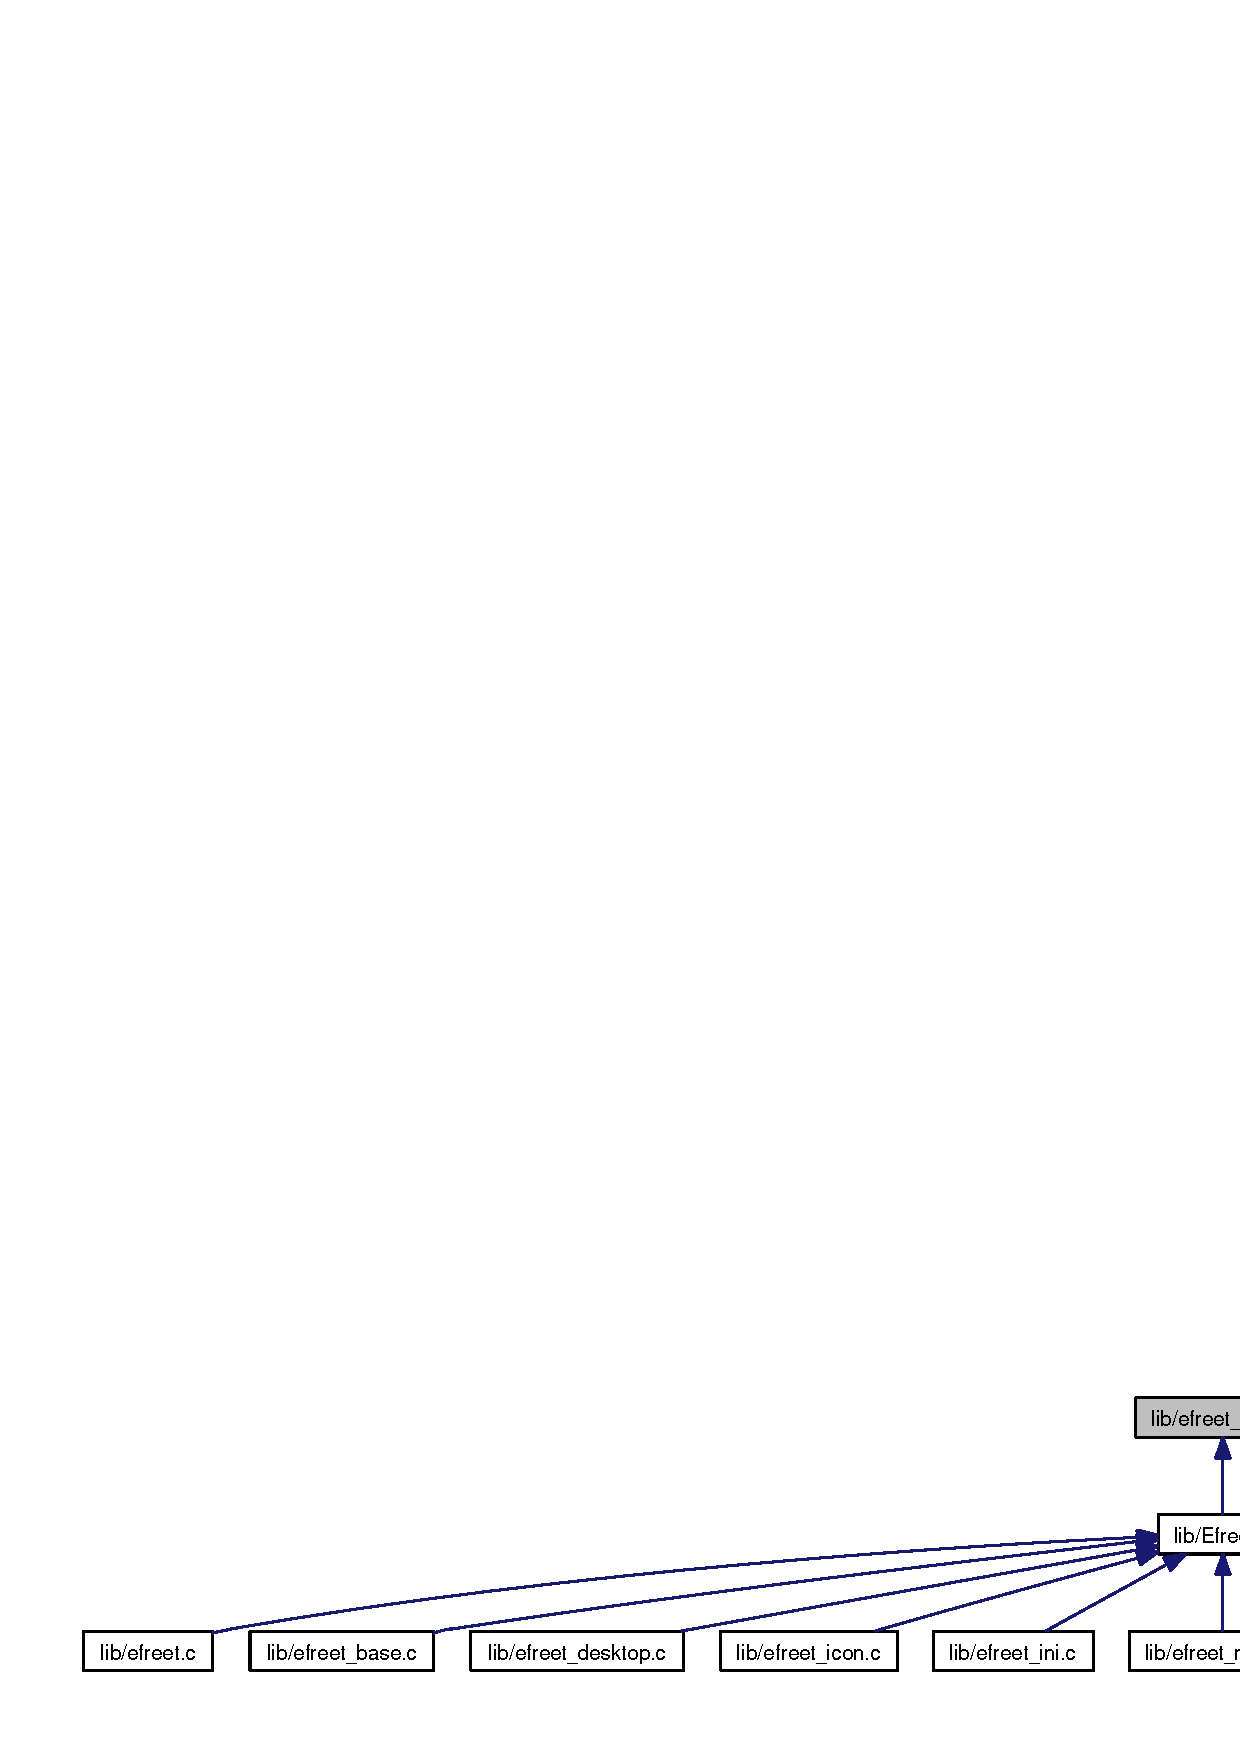
\includegraphics[width=420pt]{efreet__icon_8h__dep__incl}
\end{center}
\end{figure}
\subsection*{Data Structures}
\begin{CompactItemize}
\item 
struct {\bf Efreet\_\-Icon}
\begin{CompactList}\small\item\em Contains all the information about a given icon. \item\end{CompactList}\item 
struct {\bf Efreet\_\-Icon\_\-Point}
\begin{CompactList}\small\item\em Stores an x, y point. \item\end{CompactList}\item 
struct {\bf Efreet\_\-Icon\_\-Theme}
\begin{CompactList}\small\item\em contains all of the known information about a given theme \item\end{CompactList}\item 
struct {\bf Efreet\_\-Icon\_\-Theme\_\-Directory}
\begin{CompactList}\small\item\em Contains all the information about a sub-directory of a theme. \item\end{CompactList}\end{CompactItemize}
\subsection*{Typedefs}
\begin{CompactItemize}
\item 
typedef struct {\bf Efreet\_\-Icon} {\bf Efreet\_\-Icon}
\item 
typedef struct {\bf Efreet\_\-Icon\_\-Point} {\bf Efreet\_\-Icon\_\-Point}
\item 
typedef struct {\bf Efreet\_\-Icon\_\-Theme} {\bf Efreet\_\-Icon\_\-Theme}
\item 
typedef struct {\bf Efreet\_\-Icon\_\-Theme\_\-Directory} {\bf Efreet\_\-Icon\_\-Theme\_\-Directory}
\end{CompactItemize}
\subsection*{Enumerations}
\begin{CompactItemize}
\item 
enum {\bf Efreet\_\-Icon\_\-Size\_\-Type} \{ {\bf EFREET\_\-ICON\_\-SIZE\_\-TYPE\_\-NONE}, 
{\bf EFREET\_\-ICON\_\-SIZE\_\-TYPE\_\-FIXED}, 
{\bf EFREET\_\-ICON\_\-SIZE\_\-TYPE\_\-SCALABLE}, 
{\bf EFREET\_\-ICON\_\-SIZE\_\-TYPE\_\-THRESHOLD}
 \}
\item 
enum {\bf Efreet\_\-Icon\_\-Theme\_\-Context} \{ \par
{\bf EFREET\_\-ICON\_\-THEME\_\-CONTEXT\_\-NONE}, 
{\bf EFREET\_\-ICON\_\-THEME\_\-CONTEXT\_\-ACTIONS}, 
{\bf EFREET\_\-ICON\_\-THEME\_\-CONTEXT\_\-DEVICES}, 
{\bf EFREET\_\-ICON\_\-THEME\_\-CONTEXT\_\-FILESYSTEMS}, 
\par
{\bf EFREET\_\-ICON\_\-THEME\_\-CONTEXT\_\-MIMETYPES}
 \}
\end{CompactItemize}
\subsection*{Functions}
\begin{CompactItemize}
\item 
EAPI void {\bf efreet\_\-icon\_\-extension\_\-add} (const char $\ast$ext)
\begin{CompactList}\small\item\em Adds the given extension to the list of possible icon extensions. \item\end{CompactList}\item 
EAPI Ecore\_\-List $\ast$ {\bf efreet\_\-icon\_\-extra\_\-list\_\-get} (void)
\begin{CompactList}\small\item\em Gets the list of all extra directories to look for icons. These directories are used to look for icons after looking in the user icon dir and before looking in standard system directories. The order of search is from first to last directory in this list. the strings in the list should be created with ecore\_\-string\_\-instance(). \item\end{CompactList}\item 
EAPI {\bf Efreet\_\-Icon} $\ast$ {\bf efreet\_\-icon\_\-find} (const char $\ast$theme\_\-name, const char $\ast$icon, unsigned int size)
\begin{CompactList}\small\item\em Retrieves all of the information about the given icon. \item\end{CompactList}\item 
EAPI void {\bf efreet\_\-icon\_\-free} ({\bf Efreet\_\-Icon} $\ast$icon)
\begin{CompactList}\small\item\em Free's the given icon and all its internal data. \item\end{CompactList}\item 
EAPI char $\ast$ {\bf efreet\_\-icon\_\-list\_\-find} (const char $\ast$theme\_\-name, Ecore\_\-List $\ast$icons, unsigned int size)
\begin{CompactList}\small\item\em Retrieves all of the information about the first found icon in the list. \item\end{CompactList}\item 
EAPI char $\ast$ {\bf efreet\_\-icon\_\-path\_\-find} (const char $\ast$theme\_\-name, const char $\ast$icon, unsigned int size)
\begin{CompactList}\small\item\em Retrives the path to the given icon. \item\end{CompactList}\item 
EAPI {\bf Efreet\_\-Icon\_\-Theme} $\ast$ {\bf efreet\_\-icon\_\-theme\_\-find} (const char $\ast$theme\_\-name)
\begin{CompactList}\small\item\em Tries to get the icon theme structure for the given theme name. \item\end{CompactList}\item 
EAPI Ecore\_\-List $\ast$ {\bf efreet\_\-icon\_\-theme\_\-list\_\-get} (void)
\begin{CompactList}\small\item\em Retrieves all of the non-hidden icon themes available on the system. The returned list must be freed. Do not free the list data. \item\end{CompactList}\item 
EAPI const char $\ast$ {\bf efreet\_\-icon\_\-user\_\-dir\_\-get} (void)
\end{CompactItemize}
